%!TEX root = ../main.tex

\section{Modeling abstractions}
\label{sec:abstractions}

In this section, we introduce a running example inspired from the use-case of
Example~\ref{ex:taxes}, and describe the model abstractions that we use to
formalize the diagnosis problem.


% \ewu{Add text to say false positive complaints are an orthogonal problem.}

%!TEX root = ../main.tex


\begin{figure*}[t]
    \begin{minipage}[t]{0.28\textwidth}
         \vspace{0pt} 
         \centering
        \begin{tabular}{llll}
            \multicolumn{4}{l}{\emph{Taxes}: $D_0$}\\
            \toprule
            \textbf{ID}  & \textbf{rate}  & \textbf{income}    & \textbf{owed}\\
            \midrule
            $t_1$   & 10    & \$9500    & \$950\\
            $t_2$   & 25    & \$90000   & \$22500\\
            $t_3$   & 25    & \$86000   & \$21500\\
            \bottomrule
            \\
        \end{tabular}
    \end{minipage}
    \begin{minipage}[t]{0.43\textwidth}
         \vspace{0pt} 
         \centering
        \begin{tabular}{|p{1ex}l|}
            \multicolumn{2}{l}{\emph{Query log}: $\mathcal{Q}$}\\
            % \toprule
            \hline
            $q_1$: & \texttt{\small UPDATE Taxes SET rate = 30}\\
                   & \texttt{\small WHERE income >= \color{red}{85700}} \\
            
            $q_2$: & \texttt{\small UPDATE Taxes SET owed = income*rate/100}\\
            
            $q_3$: & \texttt{\small INSERT INTO Taxes}\\ 
                   & \texttt{\small VALUES (4, 25, 86500, 21625)}\\
            \hline
            % \bottomrule
        \end{tabular}
    \end{minipage}
    \begin{minipage}[t]{0.28\textwidth}
         \vspace{0pt} 
         \centering
        \begin{tabular}{llll}
            \multicolumn{4}{l}{\emph{Taxes}: $D_3$}\\
            \toprule
            \textbf{ID}  & \textbf{rate}  & \textbf{income}    & \textbf{owed}\\
            \midrule
            $t_1$   & 10    & \$9500    & \$950\\
            $t_2$   & 30    & \$90000   & \$27000\\
            \rowcolor{mid-gray}
            $t_3$   & \color{red}{30}    & \$86000   & \color{red}{\$25800}\\
            $t_4$   & 25    & \$86500   & \$21625\\
            \bottomrule
        \end{tabular}
    \end{minipage}

    \caption{A recent change in tax rate brackets calls for a tax rate of 30\% for those with income above \$87500.  The accounting department issues query $q_1$ to implement the new policy, but the predicate of the WHERE clause condition transposed two digits of the income value.  As a result, the tax rate of $t_3$ was increased incorrectly.  Query $q_2$ that calculates the amount owed based on the corresponding tax rate and income propagates the error.  The mistake is further obscured by query $q_3$, which inserts a tuple with similar income and the correct tax rate.}
    \label{fig:example}
\end{figure*}

\begin{example}\label{ex:taxes2}
    
Figure~\ref{fig:example} demonstrates an example tax bracket adjustment in the
spirit of Example~\ref{ex:taxes}. The adjustment sets the tax rate to 30\% for
income levels above \$87,500, and is implemented by query $q_1$. A digit
transposition mistake in the query, results in an incorrect tax rate for tuples
$t_3$ and $t_4$. Query $q_2$ that calculates the amount owed based on the corresponding
tax rate and income propagates the error to other fields. The mistake is
further obscured by query $q_3$, which inserts a tuple with slightly higher
income than $t_3$ and $t_4$ and the correct (lower) tax rate.

\end{example}
% 
While traditional data cleaning techniques seek to identify and correct the
erroneous values in the table \emph{Taxes} directly, our goal is to diagnose
the problem, and understand the reasons for these errors. In this case, the
reason for the data errors is the incorrect predicate value in query $q_1$.

In this paper, we assume that we know \emph{some} errors in the dataset, and
that these errors were caused by erroneous updates. The errors may be
obtained in different ways: traditional data cleaning tools may identify
discrepancies in the data (e.g., a tuple with lower income has higher tax
rate), or errors can be reported directly from users (e.g., customers
reporting discrepancies to customer service). \emph{Our goal is not to correct
the errors directly in the data, but to analyze them as a ``symptom'' and provide a
diagnosis.} The diagnosis can produce a targeted treatment: knowing how the
errors were introduced guides the proper way to trace and resolve them.


%!TEX root=../main.tex

\begin{figure}[t]
\centering
{\small
\begin{tabular}{ll}
    \toprule
    \textbf{Notation} & \textbf{Description}\\
    \midrule
    $\mathcal{Q}$& The sequence of executed update queries (log)\\ 
             & $\mathcal{Q}=\{q_1, \dots, q_n\}$ \\
    $D_0$    & Initial database state at beginning of log\\
    $D_n$    & End database state (current) $D_n=\mathcal{Q}(D_0)$\\
    $D_i$    & Database state after query $q_i$: $D_i=q_i(\dots q_1(D_0))$\\
    $c: t\mapsto t^*$ & Complaint: $\mathcal{T}_c(D) = (D_n\setminus\{t\})\cup\{t^*\}$\\
    $\mathcal{C}$ & Complaint set $\mathcal{C}=\{c_1,\dots,c_k\}$\\
    $\mathcal{Q}^*$& Diagnosis or log repair\\
    $d(\mathcal{Q}, \mathcal{Q}^*)$ & Distance functions between two query logs\\
    \bottomrule
\end{tabular}
}
\caption{Summary of notations used in the paper. \alex{to update once finalized}}
\label{tbl:notation}
\end{figure}

\subsection{Error modeling}
\label{sec:model}

In our setting, the diagnoses are associated with errors in the queries that
operated on the data. In Example~\ref{ex:taxes2}, the errors in the dataset
are due to the digit transposition mistake in the WHERE clause predicate of
query $q_1$. Our goal is to infer the errors in a log of queries
automatically, given a set of incorrect values in the data. We proceed to
describe our modeling abstractions for data, queries, and errors, and how we
use them to define the diagnosis problem.

\subsubsection*{Data and query models}
\label{sec:models}

\noindent
\emph{Query log ($\mathcal{Q}$):}
We define a query log that update the database 
as an ordered sequence of \texttt{UPDATE}, \texttt{INSERT}, and
\texttt{DELETE} queries $\mathcal{Q}=\{q_1,\dots,q_n\}$, that have
operated on a database $D$. In the rest of the paper, we use the term
\emph{update queries}, or just \emph{queries}, to refer to any of the queries in $\mathcal(Q)$,
including insertion and deletion queries.

\smallskip
\noindent
\emph{Query ($q_i$):} We model each query as a function over a
database $D$, resulting in a new database $D'$. For \texttt{INSERT}
queries, $D'=q(D)=D\cup\{t_{new}\}$.
We model \texttt{UPDATE} and \texttt{DELETE} queries as follows:  
\begin{align*}
    D'=q(D)= &\{\mu_{q}(t)\;|\;t\in D, \sigma_{q}(t)\}%\\
    % &
    \cup\{t\;|\;t\in D, \neg\sigma_{q}(t)\}%\\
    % &\cup\{t_{new}\;|\;q\in\texttt{INSERT}\}
\end{align*}
% 
In this definition, the modifier function $\mu_q(t)$ represents the query's update equations, and it transforms a tuple by either deleting it ($\mu_q(t)=\bot$) or changing the values of some of its attributes.
The conditional function $\sigma_q(t)$ is a boolean function that represents the query's condition predicates.  In the example of Figure~\ref{fig:example}:
\begin{align*}
    &\mu_{q_1}(t)=(30, t.income, t.owed)\\
    &\sigma_{q_1}(t)=(t.income\ge 85700)\\
    &\mu_{q_2}(t)=(t.rate, t.income, \frac{t.income\cdot t.rate}{100})\\
    &\sigma_{q_2}(t)=\texttt{true}
\end{align*} 
Note that in this paper, we only consider query without sub-query or aggregation. 
% 
% As an insertion query, $q_3$ has $\sigma_{q_3}(t)=\texttt{false}$ and $t_{new}=(25, 85800, 21450)$.
% \ewu{why does it return false?  should it only be true if input is $\bot$?}


\smallskip
\noindent
\emph{Database state ($D_i$):}
We use $D_i$ to represent the state of a database $D$ after the application of
queries $q_1$ through $q_i$ from the log $\mathcal{Q}$. $D_0$ represents the
original database state, and $D_n$ the final, or current, database state. Out
of all the states, the system only maintains $D_0$ and $D_n$. In practice,
$D_0$ can be a checkpoint: a state of the database that we assume is correct;
we cannot diagnose errors before this state. The intermediate states can be
derived by executing the log: $D_i=q_i(q_{i-1}(\dots q_1(D_0)))$. We also
write $D_n=\mathcal{Q}(D_0)$ to denote that the final database state $D_n$ can
be derived by applying the sequence of queries in the log to the original
database state $D_0$.

\smallskip
\noindent
\emph{True database state ($D_i^*$):}
Queries in $\mathcal{Q}$ are possibly erroneous, introducing errors in the
data. There exists a sequence of \emph{true} database states $\{D_0^*,
D_1^*\dots, D_n^*\}$, with $D_0^*=D_0$, representing the database states that
would have occurred if there had been no errors in the queries.
The true database states are unknown; our goal is to find and correct the errors in $\mathcal{Q}$ and retrieve the correct database state $D_n^*$.

For ease of exposition, in the remainder of the paper we assume that the
database contains a single relation with attributes $A_i,\ldots,A_m$,
but the single table is not a requirement in our framework.


\subsubsection*{Error models}

Following the terminology in Examples~\ref{ex:telco}
and~\ref{ex:taxes}, we model a set of identified or user-reported
data errors as \emph{complaints}. A complaint corresponds to a
particular tuple in the final database state $D_n^*$, and identifies
that tuple's correct value assignment. We formally define complaints
below:

\begin{definition}[Complaint]
    A complaint $c$ is a mapping between two tuples: $c: t\mapsto t^*$, such that $t$ and $t^*$ have the same schema, $t\in D_n\cup\{\bot\}$, and $t\neq t^*$. A complaint defines a
    transformation $\mathcal{T}_c$ on a database state $D$: $\mathcal{T}_c(D)
    = (D\setminus\{t\})\cup\{t^*\}$.
\end{definition}

In the example of Figure~\ref{fig:example}, two complaints are reported on the final database state $D_3$: 
$c_1: t_3\mapsto t_3^*$ and
$c_2: t_4\mapsto t_4^*$, where $t_3^*=(25,86000,21500)$
and $t_4^*=(25,86500,21625)$.  For both these cases, each complaint denotes a value correction for a tuple in $D_3$.  Complaints can also model the addition or removal of tuples: $c: \bot\mapsto t^*$ means that $t^*$ should be added to the database, whereas $c: t\mapsto \bot$
means that $t$ should be removed from the database.


\smallskip
\noindent
\emph{Complaint set ($\mathcal{C}$):}
We use $\mathcal{C}$ to denote the set of all known complaints
$\mathcal{C}=\{c_1,\dots,c_k\}$, and we call it the \emph{complaint set}.
Each complaint in $\mathcal{C}$ represents a transformation (addition,
deletion, or modification) of a tuple in $D_n$. We assume that the
complaint set is consistent, i.e., there are no two complaints that
propose different transformations to the same tuple $t\in D_n$.
Applying all these transformations to $D_n$ results in a new database
instance
$D_n'=\mathcal{T}_{c_1}(\mathcal{T}_{c_2}(\dots\mathcal{T}_{c_k}(D_n)))$.\footnote{Since
the complaint set is consistent, it is easy to see that the order of
transformations is inconsequential.} $\mathcal{C}$ is \emph{complete}
if it contains a complaint for each error in $D_n$. In that case,
$D_n'=D_n^*$. In our work, we do not assume that the complaint set is
complete, but, as is more common in practice, we only know a subset of
the errors (incomplete complaint set). Further, we focus our analysis
on \emph{valid} complaints; we briefly discuss dealing with invalid
complaints (complaints identifying a correct value as an error) in
Section~\ref{sec:noise}, but these techniques are beyond the scope of this paper.

\smallskip
\noindent
\emph{Log repair ($\mathcal{Q}^*$):}
The goal of our framework is to derive a diagnosis as a log repair
$\mathcal{Q}^*=\{q_1^*,\dots, q_n^*\}$, such that
$\mathcal{Q}^*(D_0)=D_n^*$. In this work, we focus on errors produced
by incorrect parameters in queries, so our repairs focus on altering
query constants rather than query structure. Therefore, for each query
$q_i^*\in\mathcal{Q}^*$, $q_i^*$ has the same structure as $q_i$
(e.g., the same number of predicates and the same variables in the \texttt{WHERE} clause), 
but possibly different parameters. For example, a good log repair for the
example of Figure~\ref{fig:example} is
$\mathcal{Q}^*=\{q_1^*,q_2,q_3\}$, where $q_1^*$=\texttt{UPDATE Taxes
SET rate = 30 WHERE income >= 87500}.


\subsubsection*{Problem definition}

We now formalize the problem definition for diagnosing data
errors using query logs. A diagnosis is a log repair
$\mathcal{Q}^*$ that resolves all complaints in the set $\mathcal{C}$
and leads to a correct database state $D_n^*$.

\begin{definition}[Optimal diagnosis]\label{def:problem}
    Given database states $D_0$ and $D_n$, a query log $\mathcal{Q}$ such that $\mathcal{Q}(D_0)=D_n$, a set of complaints $\mathcal{C}$ on $D_n$,  and a distance function $d$, the optimal diagnosis is a log repair $\mathcal{Q}^*$, such that:
    \begin{itemize}[itemsep=0pt, parsep=0pt]
        \item $\mathcal{Q}^*(D_0)=D_n^*$, where $D_n^*$ has no errors
        \item $d(\mathcal{Q}, \mathcal{Q}^*)$ is minimized
    \end{itemize}
\end{definition}

More informally, we seek the minimum changes to the log $\mathcal{Q}$
that would result in a clean database state $D_n^*$. Obviously, a
challenge is that $D_n^*$ is unknown, unless we know that the
complaint set is complete. 

In Section~\ref{sec:sol}, we describe our basic method $\sys_{naive}$, 
which
uses a constraint programming formulation that expresses this
diagnosis problem as a mixed integer linear program (MILP). 
% We justify
% using this constraint formulation as opposed to methods, such as
%classification, that can analyze one query at a time in Section~\ref{sec:heuristic}. We show that the latter, heuristic
% approach is flawed, and one needs to encode the constraints in the entire log.
In Section~\ref{sec:opt}, we present several optimization
techniques that extend our naive method, allowing \sys to (1)~handle
cases of incomplete information (incomplete complaint set), and
(2)~scale to large data and log sizes. Specifically, the proposed \sys algorithm with incremental
repair optimization (Section~\ref{sec:incremental}), can
handle $10\times$ compared to the basic MILP approach.


% \begin{figure}[t]
% \centering
% 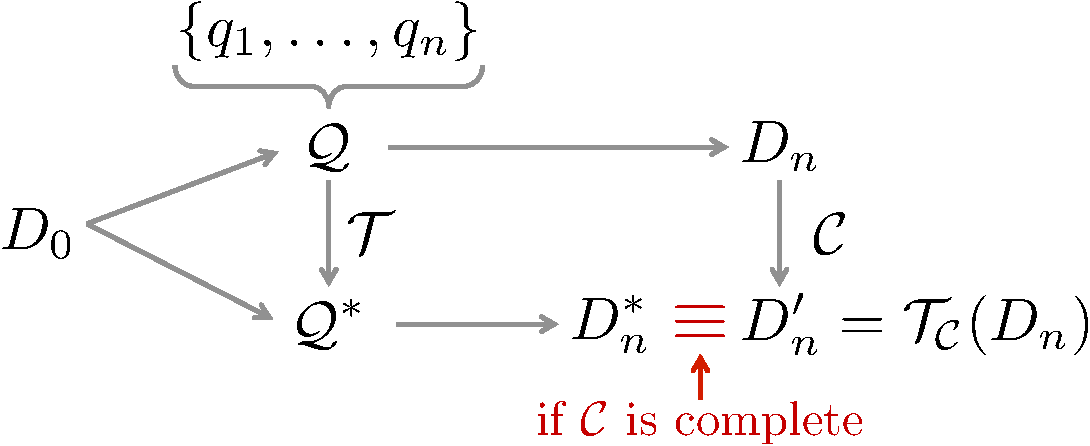
\includegraphics[width = 0.75\columnwidth]{figures/probtransform}
% \caption{Graphical depiction of the diagnosis problem in our \sys framework.  $D_0$, $D_n$, $\mathcal{Q}$, and $\mathcal{C}$ are given, and \sys uses them to derive the log repair $\mathcal{Q}^*$.
% \alex{not sure if this figure is actually useful.}}
% \label{f:probtransform} 
% \end{figure}


% \deprecate{
% \subsection{Naive Formulation}
% 
% The most general version of the problem
% (depicted in Figure~\ref{f:probtransform}) is to find a sequence of
% transformations $T$ that insert, delete, and/or modify queries in $Q_{seq}$ 
% such that the resulting sequence, $Q'_{seq} = T(Q_{seq})$, resolves the user's complaint set. 
% 
% However this problem is ill-defined because there exist an unbounded set of transformations that
% can resolve the user's complaint set.  A naive solution is to append to the query log a statement
% that deletes all the records in the database, followed by a query that insert all of the correct records.
% Unfortunately this naive solution does not help explain the complaints in any way!
% 
% \subsection{Constraints}
% 
% For this reason, we constrain the set of possible transformations $\mathcal{T}$ to the following:
% 
% \begin{itemize}
% \item delete query
% \item modify insert statement constants
% \item modify constants in WHERE clause
% \end{itemize}
% 
% Our transformations don't include adding new queries, synthesizing arbitrary queries, or modifying the
% number of clauses in a WHERE condition.  We apply these restrictions because we believe it is more likely
% for the user to mis-type a constant value as opposed to having an error in the query structure.
% 
% Futhermore we define a distance metric between two query logs in order to evaluate
% the qulatiy of a transformation.
% \xxx{define $\mathcal{T}$ here.}
% 
% 
% 
% \subsection{Problem Statements}
% 
% In this paper, we present three variants of this problem.
% 
% \begin{problem}[Prob-Complete]\label{prob:complete}
% Given $C = P_{D_n, D^*_n}$, $Q_{seq}$, and the sequence of database states $D_0,\ldots,D_n$, 
% identify a sequence of transformations $T$ such that:
% \begin{itemize}
% \item $T(Q_{seq})(D_0) = C(D_n)$
% \item $|T| = 1$
% \item $T$ metric is minimized
% \end{itemize}
% \end{problem}
% 
% This variation of the problme relaxes the constraint that the complaint set must be complete, and allows
% for both false positives as well as false negatives.  The goal is the same, however the constraints are relaxed:
% 
% \begin{problem}[Prob-Incomplete]\label{prob:incomplete}
% Given $C$ where $acc_C < 1$, $Q_{seq}$, and the sequence of database states $D_0,\ldots,D_n$, 
% identify a sequence of transformations $T$ such that:
% \begin{itemize}
% \item $T(Q_{seq})(D_0) = D^*_n$
% \item $T$ metric is minimized.
% \item $|T| = 1$
% \end{itemize}
% \end{problem}
% 
% Finally, we extend the problem to allow transformations with one or more operations.
% 
% \begin{problem}[Prob-MultiQ]\label{prob:multi}
% Given $C$ where $acc_C < 1$, $Q_{seq}$, and the sequence of database states $D_0,\ldots,D_n$, 
% identify a sequence of transformations $T$ such that:
% \begin{itemize}
% \item $T(Q_{seq})(D_0) = D^*_n$
% \item $T$ metric is minimized.
% \end{itemize}
% \end{problem}
% 
% 
% 
% 
% \subsection{A Naive Approach}
% 
% \begin{itemize}
% \item roll back complaints to penultimate state using algebraic expressions 
% \item perturb each expression in query until the query result matches correct state
% \item if an expression cannot be found, iterate
% \end{itemize}
% 
% 
% Not clear how to roll back complaints
% 
% Ways to perturb query expressions is unbounded
% 
% }